The problem of machines-teaching-machines has become an interesting topic in machine learning area. This problem focuses on how to let the student machines learn from their teacher machines effectively, in addition to training data.

Similar to our human teaching scenario, a typical paradigm for this problem is using the intelligent teacher to provide privileged information for the student model in the learning process while the student model has no access to the privileged information at the test time \cite{vapnik2009new}\cite{vapnik2015learning}. On the other hand, using the soft output from an ensemble of models to train a single model, known as \textit{Distillation} demonstrates its ability to transfer the knowledge between models in many real world applications  \cite{Gupta_2016_CVPR}\cite{hinton2015distilling}\cite{luo2016face}\cite{Tzeng_2015_ICCV}\cite{urban2016deep}. 

A recent framework unifies this two approaches together and train the student model by distilling the knowledge from a teacher model trained with privileged information, which is referred to as \textit{Generalized Distillation} \cite{lopez2015unifying}. This framework can be applied to many learning tasks, such as semi-supervised learning and multi-task learning. It is reasonable to apply Generalized Distillation to \textit{Domain Adaptation}, called \textit{Generalized Distillation Domain Adaptation} (\textbf{GDDA}), where we treat the source model as the teacher model to provide the soft label for the examples in the target domain in the training process to train the model for the target domain.  
There are several advantages for GDDA,
such as compatible with various of classifiers and scenarios, highly effective in small data regimes (For more details, see Section \ref{sec:gdda}).

In Generalized Distillation, the imitation parameter controls the importance of the teacher model. Accordingly, in GDDA, the imitation parameter controls the amount of the knowledge transferred from the source model. We show that the imitation parameter determines the quality of the transfer process, i.e. the performance of the target model (see Section \ref{sec:gdda}). In previous work, this imitation parameter can only be determined  by either brute force search or background knowledge \cite{lopez2015unifying}\cite{Tzeng_2015_ICCV}. It is not clear how to determine the value of imitation parameter effectively, which become more crucial especially for the multi-source scenario in domain adaptation, where there could be multiple imitation parameters to be determined.

\begin{figure}
\centering
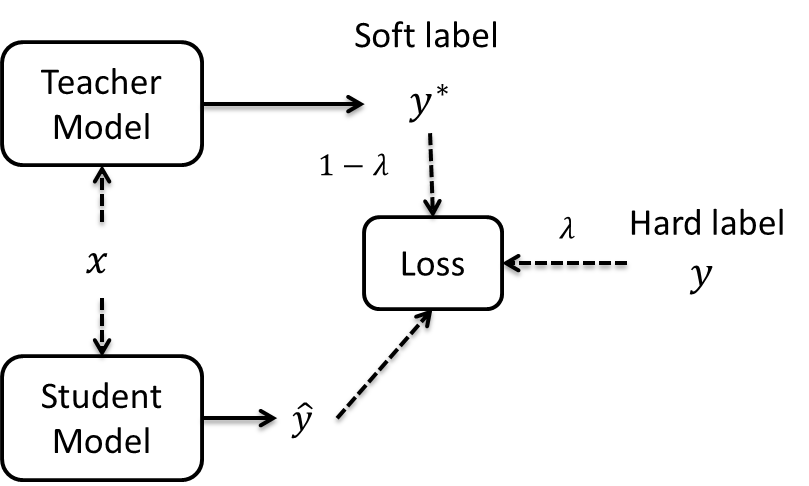
\includegraphics[scale=.8]{figure/GDDA.png}
\caption{Illustration of GDDA training process.}
\end{figure}
In this paper, we propose a novel method for GDDA, called GDDA-SVM that can determine the imitation parameter automatically. In particular, inspired by \cite{cawley2006leave}, we use $\ell_2-$loss for GDDA-SVM and show that the Leave-one-out cross validation (LOOCV) loss can be calculated in a closed form. By minimizing the LOOCV loss on the target training data, we can find the optimal imitation parameter for the target model. In our experiments, we show that GDDA-SVM can effectively find the optimal imitation parameter and achieve better performance compared to methods using brutal force search. The main contributions of this paper include: (1) We propose the framework GDDA for domain adaptation. (2) We propose a method GDDA-SVM for imitation parameter estimation.

The rest of this paper is organized as follow: In Section \ref{sec:work}, we describe the related work on privileged information and distillation in domain adaptation. Section \ref{sec:gdda} we propose our framework of GDDA and provide some statistic analysis. Based on that, we propose our GDDA-SVM in Section \ref{sec:svm}. Experimental results are shown in Section \ref{sec:exp}. Some discussion and conclusion are provided in Section \ref{sec:con}.

%For our human, a good student can learn a new concept very fast under the supervision of the teacher with just a few examples and make meaningful generalizations to novel instances. 